% This is the preamble

\documentclass[a4paper]{article}
\usepackage[margin=1in]{geometry}

\usepackage{fancyhdr}
\pagestyle{fancy}
\lhead{Convolution Investigation}
\rhead{\thepage}
\renewcommand{\headrulewidth}{0.4pt}
\renewcommand{\footrulewidth}{0.4pt}

\usepackage{mathtools}
\DeclarePairedDelimiter{\ceil}{\lceil}{\rceil}
\DeclarePairedDelimiter\floor{\lfloor}{\rfloor}

\usepackage[utf8x]{inputenc}
\usepackage{amsmath} % For math formatting
\usepackage{graphicx}
\usepackage{hyperref} 
\usepackage{tcolorbox}
\usepackage{commath}
\usepackage{xcolor}
\hypersetup{
    colorlinks,
    linkcolor={red!50!black},
    citecolor={blue!50!black},
    urlcolor={blue!80!black}
}
\usepackage{multicol}
\usepackage{amssymb}

\newcommand{\op}[2]{#1\{#2\}}

\title{Understanding Convolution}
\author{David Egolf}
\date{September 12, 2016}
% Where the document starts
\begin{document}
\maketitle

\section*{Definition}
The convolution of two sequences $x[n]$ and $h[n]$:
\begin{align*}
(x*h)[n] = \sum_{k=-\infty}^{\infty}x[k]h[n-k]
\end{align*}
Intuitively, we are placing a shifted copy of the sequence $h$ centered at $x = k$, and multiplying this by the $k_{th}$ element in the sequence $x[n]$. We do this for all elements $x[k]$ in the input sequence and add the results.
\\\\
Note that convolution is commutative, distributive, and associative.
\section*{Output of LTI System}
Assume $T$ is a linear time invariant system. Then:
\begin{align*}
\op{T}{\delta[n]} &= h[n] \text{ (impulse response)}\\
\implies \op{T}{x[n]} &= \sum_{k=-\infty}^{k=\infty}x[k]h[n-k]
\end{align*}
\subsection*{Non-linearity of Auto-Correlation and Convolution}
We begin with self convolution (SC), with $A, B \in \mathbb{C}$:
\begin{align*}
((A \cdot h+B \cdot g)*(A \cdot h+B \cdot g))[n] &= \sum_{k = -\infty}^{\infty} (A \cdot h+B \cdot g)[k] \cdot (A \cdot h+B \cdot g)[n-k] \\
&= \sum_{k = -\infty}^{\infty} (A \cdot h[k]+B \cdot g[k]) \cdot (A \cdot h[n-k]+B \cdot g[n-k]) \\
&= \sum_{k = -\infty}^{\infty} A^2  h[k]h[n-k]+B^2 g[k]g[n-k] + A \cdot B \cdot h[k]g[n-k] + A \cdot B \cdot g[k]h[n-k] \\
&= A^2(h*h)[n] + B^2(g*g)[n] + A \cdot B \cdot ((h*g)[n] + (g*h)[n])
\end{align*}
So, self convolution is in general not a linear operation. Note also that unless $(h*g)[n] = 0$, then we can't have $(h*g)[n] = -(g*h)[n]$. This is because convolution is commutative.
\\\\
We are therefore interested in finding nonzero sequences that have zero convolution. Looking on Google, one can find examples of such sequence pairs, although it appears that at least one of the sequences in the pair needs to have nonzero values arbitrarily far out. While this is interesting, it looks probably difficult to use this to exploit this pseudo linear property of self convolution.
\\\\
Considering now autocorrelation:
\begin{align*}
((A \cdot h+B \cdot g)\star(A \cdot h+B \cdot g))[n] &= \sum_{k = -\infty}^{\infty} (A \cdot h+B \cdot g)[k] \cdot (A \cdot h+B \cdot g)[k-n] \\
&= \sum_{k = -\infty}^{\infty} (A \cdot h[k]+B \cdot g[k]) \cdot (A \cdot h[n-k]+B \cdot g[k-n]) \\
&= \sum_{k = -\infty}^{\infty} A^2  h[k]h[n-k]+B^2 g[k]g[k-n] + A \cdot B \cdot h[k]g[k-n] + A \cdot B \cdot g[k]h[k-n] \\
&= A^2(h\star h)[n] + B^2(g \star g)[n] + A \cdot B \cdot ((h\star g)[n] + (g \star h)[n])
\end{align*}
So, autocorrelation is similarly not linear.
\section*{Model Ultrasound System as LTI System}
Consider a single ultrasound transducer, and assume that we use it to transmit a signal, which is then reflected and received by the transducer. Let us define an ultrasound system $U$ that maps from transducer input excitation to the final signal decoded by the transducer:
\begin{align*}
U = T_x \circ M_x \circ R_x
\end{align*}
where $T_x$ is the transmission operator, $M_x$ is the reflection operator (acts like a ``mirror"), and $R_x$  is the receiving operator.
\\\\
If we ignore the transmission delay, and assume that the reflected signal is identical to the transmitted signal up to a change in amplitude, then:
\begin{align*}
\op{M_x}{x[n]} = A \cdot x[n]
\end{align*}
where $A \in \mathbb{R}$.
\\\\
In our simulations we assume that the both $T_x$ and $R_x$ are LTI systems, with the same impulse response. Call this common transducer impulse response $h$. 
\\\\
Using these definitions, we can calculate the output of the ultrasound system:
\begin{align*}
\op{U}{x[n]} &= \op{T_x \circ M_x \circ R_x}{x[n]} \\
&= h[n] *(A \cdot h[n] * x[n]) \\
&= A \cdot \ (h[n] * h[n]) *x[n]
\end{align*}
where we have used the fact that convolution is commutative.
\clearpage
\subsection*{Motivation}
So, in order to understand the action of the ultrasound system, it would be useful to understand the properties of $h[n] * h[n]$, since this is the impulse response of the entire system (up to a scalar multiple).
\section*{Problem Statement}
Investigate the properties of  the self convolution $(h*h)[n]$ of a sequence $h: \mathbb{Z} \rightarrow \mathbb{R}$, in the context of an ultrasound system.
\section*{Solution}
\subsection*{Causal}
I assume there is no noise in the ultrasound system to be modeled. I assume that in a noise free ultrasound system, the system will not begin to transmit data prior to excitation, and the system will not begin to receive data prior to a transmitted signal hitting the receiver. Therefore:
\begin{align*}
h[n] = 0 \text{ for } n < 0 \implies (h*h)[n] = 0 \text{ for } n < 0 
\end{align*}
This implies that the LTI system  $h*h$ is causal. 
\subsection*{Stable}
I assume that if we stop exciting the transducer, then after a finite amount of time the ultrasound receiver will stop receiving anything. That is:
\begin{align*}
(h*h)[n] = 0 \text{ for } n \geq N
\end{align*}
This implies that we are working with a finite impulse response system, and therefore the system is stable.
\subsection*{Not Memory-less}
The output $y[n]$ depends on all values of the input $h[n]$, not just the current value of $n$. Therefore, the system is not memory-less.
\subsection*{Equation for Output}
The output of the system $(h*h)[n]$ is explicitly:
\begin{align*}
(h*h)[n] &= \sum_{k=-\infty}^{\infty}h[k]h[n-k]
\end{align*}
Since the system is causal, we only need to sum over the terms where $k \geq 0$ and $n - k \geq 0 \implies k \leq n$:
\begin{align*}
(h*h)[n] &= \sum_{k=0}^{n}h[k]h[n-k]
\end{align*}
To get some intuition, we write out this sum explicitly in the case when $h[0] = 1, h[1] = 2, h[2] = 3, h[3] = 4, h[4] = 5$ and $h[j] = 0$ for all other $j \in \mathbb{Z}$:
\begin{align*}
(h*h)[n] &= h[0]h[n] + h[1]h[n-1] + h[2]h[n-2] + h[3]h[n-3] + h[4]h[n-4]
\end{align*}
\clearpage
\subsection*{Nonzero Output Region As Function of Length}
Let $L$ be an integer called the ``length" of the impulse response. We provide elements $h[0], h[1], ..., h[L-1]$ to MATLAB when specifying the impulse response. We require $L \geq 1$ and $h[n] = 0$ for all $n \geq L$.
\\\\
We assume that our impulse response starts at zero and ends at zero, so set $h[0] = h[L-1] = 0$.
\\\\
Using this information, we can rewrite the form of the output $(h*h)[n]$. We are interesting in determining exactly at which times the output can be nonzero. The output $(h*h)[n]$ will be zero at $n$ if:
\begin{align*}
h[k]h[n-k] = 0 \text{ for } k = 0,1,..,n
\end{align*}
Since we assume $h[0] = 0$ and $(h*h)[n] = 0$ for all $n \geq L -1$, we can reduce the number of terms under consideration. Specifically, if $n \geq L-1$, then the output is zero, and if $n \leq 0$ then the output is zero. So, it remains to consider the cases in which $1 \leq n \leq L -2$. These are the only cases in which would possibly get nonzero output.
\\\\ 
We can further restrict these cases by realizing that if $L \leq 2$, then the entire sequence is zero and so the output will be zero. So, we only need to consider the cases $1 \leq n \leq L -2$ where $L \geq 3$. We want to know for which of these $n$ values we have a chance for nonzero output, as a function of $L$ (clearly the maximum $n$ for nonzero output will increase with $L$).
\\\\
Our strategy is to start small and search for a pattern:
\\\\
If $n = 1$:
\begin{align*}
h[k]h[n-k] = h[k]h[1-k]
\end{align*}
Since $1 - k \leq 0$ for $k = 1,..,L-2$, the output is always zero in this case. As a result, we only need to consider the possible nonzero cases as consisting of $2 \leq n \leq L -2$.
\\\\
If $n = 2$:
\begin{align*}
h[k]h[n-k] = h[k]h[2-k] \\
\end{align*}
The possible nonzero $h[i]$ range is $i = 1,2..,L-2$. Checking when we are in this range:
\begin{align*}
1 \leq 2-k \leq L -2 \\
\implies k &\leq 1 \text{ and}\\
\implies 4 &\leq L + k \implies k \geq 4 - L \\
\text{Together: } \\
4 - L \leq k \leq 1
\end{align*}
In order to satisfy this inequality, we need:
\begin{align*}
4 - L \leq 1 \implies L \geq 3
\end{align*}
We also need:
\begin{align*}
4 - L  \leq k_{max}, 1  \geq k_{min}
\end{align*}
Where $k_{max}$ is the largest value $k$ can take on, and $k_{min}$ is the smallest value $k$ can take on, while preserving the fact that $h[k]$ might be nonzero. From our work before, $k_{max} = L - 2$ and $k_{min} = 1$.
\\\\
So, we need:
\begin{align*}
4 - L \leq L -2, 1 \geq 1 \\
\implies 2L \geq 6 \implies L \geq 3
\end{align*}
\\\\
So, $(h*h)[2]$ has a chance to be nonzero when $L \geq 3$.
\clearpage
Let's generalize this argument, setting $n = a$:
\begin{align*}
h[k]h[n-k] = h[k]h[a-k] \\
\end{align*}
The possible nonzero $h[i]$ range is $i = 1,2..,L-2$. Checking when we are in this range:
\begin{align*}
1 \leq a-k \leq L -2 \\
&\implies k \leq a - 1 \text{ and}\\
&\implies a + 2 \leq L + k \implies k \geq a + 2 - L \\
\text{Together: } \\
a + 2 - L \leq k \leq a - 1
&\implies L \geq 3
\end{align*}
We also need:
\begin{align*}
a + 2 - L  \leq k_{max}, a - 1  \geq k_{min}
\end{align*}
Where $k_{max}$ is the largest value $k$ can take on, and $k_{min}$ is the smallest value $k$ can take on, while preserving the chance that $h[k]$ might be nonzero. From our work before, $k_{max} = L - 2$ and $k_{min} = 1$.
\\\\
So, we need:
\begin{align*}
a +2 - L \leq L -2,~a-1 \geq 1 \implies a \geq 2 \\
\implies 2L \geq a + 4 \implies L \geq \frac{a+4}{2}
\end{align*}
\\\\
Substituting $n = a$, we find $(h*h)[n]$ has a chance to be nonzero when $L \geq \frac{n+4}{2}$ and when $n \geq 2$.
\\\\
\subsection*{Largest and Smallest Nonzero $(h*h)[n]$}
Using this information, we can find the first possibly nonzero term. Trying $n = 2$, the condition for the output to be nonzero is:
\begin{align*}
L \geq \frac{2+4}{2} = 3 \implies L \geq 3
\end{align*}
So, $n = 2$ is the smallest value of $n$ for which $(h*h)[n]$ is possibly not zero. 
\\\\
Next, let's find the largest $n = n_{max}$ for which $(h*h)[n]$ is possibly nonzero. We know that this $n \geq 2$. Also, for $(h*h)[n_{max}]$ to be possibly nonzero, we need:
\begin{align*}
2L \geq n_{max} + 4 \\ 
\implies n_{max} \leq 2L - 4
\end{align*}
Choosing the largest element in this set, we get $n_{max} = 2L -4$.
\\\\
So, $(h*h)[n]$ is possibly nonzero for $2 \leq n \leq 2L-4$.
\subsection*{Properties of $h*h$ So Far}
Adding this new information about the nonzero range for $n$:
\begin{align*}
(h*h)[n] = \sum_{k=0}^{n}h[k]h[n-k] \text{ (possibly nonzero for } 2 \leq n \leq 2L-4) 
\end{align*}
This system is LTI, causal, stable, and not memory-less.
\clearpage
\subsection*{Lack of Symmetry in Self Convolution}
It turns out that the convolution of a sequence with itself is NOT symmetric (doesn't form a palindrome when written out), even though the autocorrelation of a sequence with itself is! For example, if $h = [0,1,2,0]$ (starting at $n = 0$), then:
\begin{align*}
(h*h)[0]& = \sum_{k=0}^{0}h[k]h[0-k] = h[0]h[0] = 0 \\
(h*h)[1] &= \sum_{k=0}^{1}h[k]h[1-k] = h[0]h[1] + h[1]h[0] = 0 \\
(h*h)[2] &= \sum_{k=0}^{2}h[k]h[2-k] = h[0]h[2] + h[1]h[1]+h[2]h[0]= 0 + 1 + 0 = 1 \\
(h*h)[3] &= \sum_{k=0}^{3}h[k]h[3-k] = h[0]h[3] + h[1]h[2]+h[2]h[1]+h[3]h[0]= 0 + 2 + 2 + 0 = 4 \\
(h*h)[4] &= \sum_{k=0}^{4}h[k]h[4-k] = h[0]h[4] + h[1]h[3]+h[2]h[2]+h[3]h[1] + h[4]h[0]= 0 + 0 + 4 + 0 = 4 \\
\end{align*}
And since $n_{max} = 2L-4 = 4$, $(h*h)[n] = 0$ for all larger $n$.
\subsection*{Sufficient Condition for Symmetry in Self Convolution}
The autocorrelation of a sequence is known to be symmetric. The autocorrelation for a real sequence is:
\begin{align*}
ACF(h[n]) = \sum_{k=-\infty}^{\infty}h[k]h[k-n]
\end{align*}
For comparison, here is the the definition of a sequence convolved with itself:
\begin{align*}
(h*h)[n] &= \sum_{k=-\infty}^{\infty}h[k]h[n-k] \\
&= \sum_{k=-\infty}^{\infty}h[k]h[-(k-n)]
\end{align*}
If we assume that $h[n]$ satisfies $h[n] = h[-n]$ (it is symmetric in time), then $h[-(k-n)] = h[n-k]$ and we find $ACF(h[n]) = (h*h[n])$ in this case. So, a time symmetric sequence $h[n] = h[-n]$ has a symmetric self convolution.
\subsection*{Incorporating Sinusoidal Shape}
The impulse function $h[n]$ we use in simulation is of the form:
\begin{align*}
h[n] = a[n]\sin(w \cdot n)
\end{align*}
where $a[n]$ is a sequence of real numbers and $w \in \mathbb{R}$. I assume that we use  a natural number $m$ of cycles (in order to ensures that $h[0] = h[L-1] = 0$ and also to produce an output that integrates to zero - which helps reduce side lobe energy). This tells us the value of $w$:
\begin{align*}
w \cdot (L-1) = 2 \pi m \\
\implies w = \frac{2 \pi m}{L-1}
\end{align*}
So, the impulse $h[n]$ is of the form, where $m \in \mathbb{N}$ is the number of cycles used:
\[
 h[n] =
  \begin{cases} 
      \hfill a[n]\sin(\frac{2 \pi m}{L-1} \cdot n)   \hfill & 0 \leq n \leq L -1 \\
      \hfill 0 \hfill & \text{ for all other $n$} \\
  \end{cases}
\]
\clearpage
\subsection*{Consequences of Sinusoidal Shape}
For simplicity, we begin by assuming $a[n] = 1$ for all $n$. MATLAB evidencce seems to suggest that with the additional assumption of sinusoidal shape, the impulse response of the ultrasound system $h*h$ is now symmetric:
\begin{center}
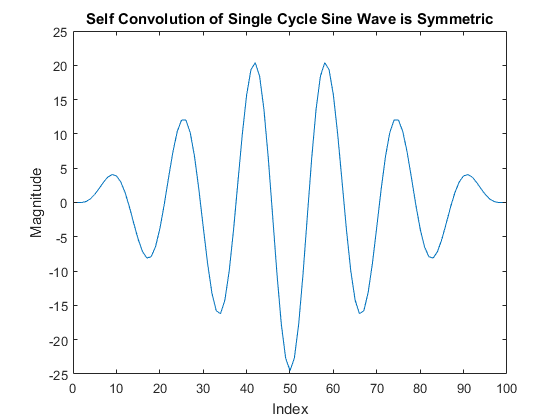
\includegraphics[scale=1]{symmConvSin.png}
\end{center}
The reason we get a symmetric self convolution with a negative peak  is that our sine wave excitation has odd symmetry about its center:
\begin{align*}
h[a] = -h[L-1 - a]~\forall a \in \mathbb{Z} \\
\end{align*}
So, in a sine wave, as we come in from the left, we find a value negative of what we find as we come in from the right.
(ASSUMED FOR NOW) \\\\
As a consequence of this symmetry, then $h*h$ is the negative of the autocorrelation of $h$. As a result, $h*h$ has a negative peak and is symmetric about the center of its nonzero values.
\\\\
To see why this is the case, note that the definition of autocorrelation of $h$ corresponds to fixing one copy of $h$ and sliding another copy of $h$ past it to the right, multiplying vertically and then summing:
\begin{align*}
ACF(h[n]) = \sum_{k=-\infty}^{\infty}h[k]h[k-n]
\end{align*}
Here, $h[k]$ is the unshifted copy, and $h[k-n]$ is the copy which is shifted by $n$.
\\\\
The self convolution is really similar:
\begin{align*}
(h*h)[n] = \sum_{k=-\infty}^{\infty}h[k]h[n-k] =  \sum_{k=-\infty}^{\infty}h[k]h[-(k-n)]
\end{align*}
In this case, we fix one copy of $h$ and slide a horizontally flipped copy of $h$ past it to the right, multiplying vertically and then summing.
\clearpage
The following figure shows that summing over $h[-(k-n)]$ consists of summing over reversed shifted copies of $h[n]$ (source ``Artificial Intelligence" on GitBook, by Leonardo Araujo dos Santos):
\begin{center}
\begin{figure}[h]
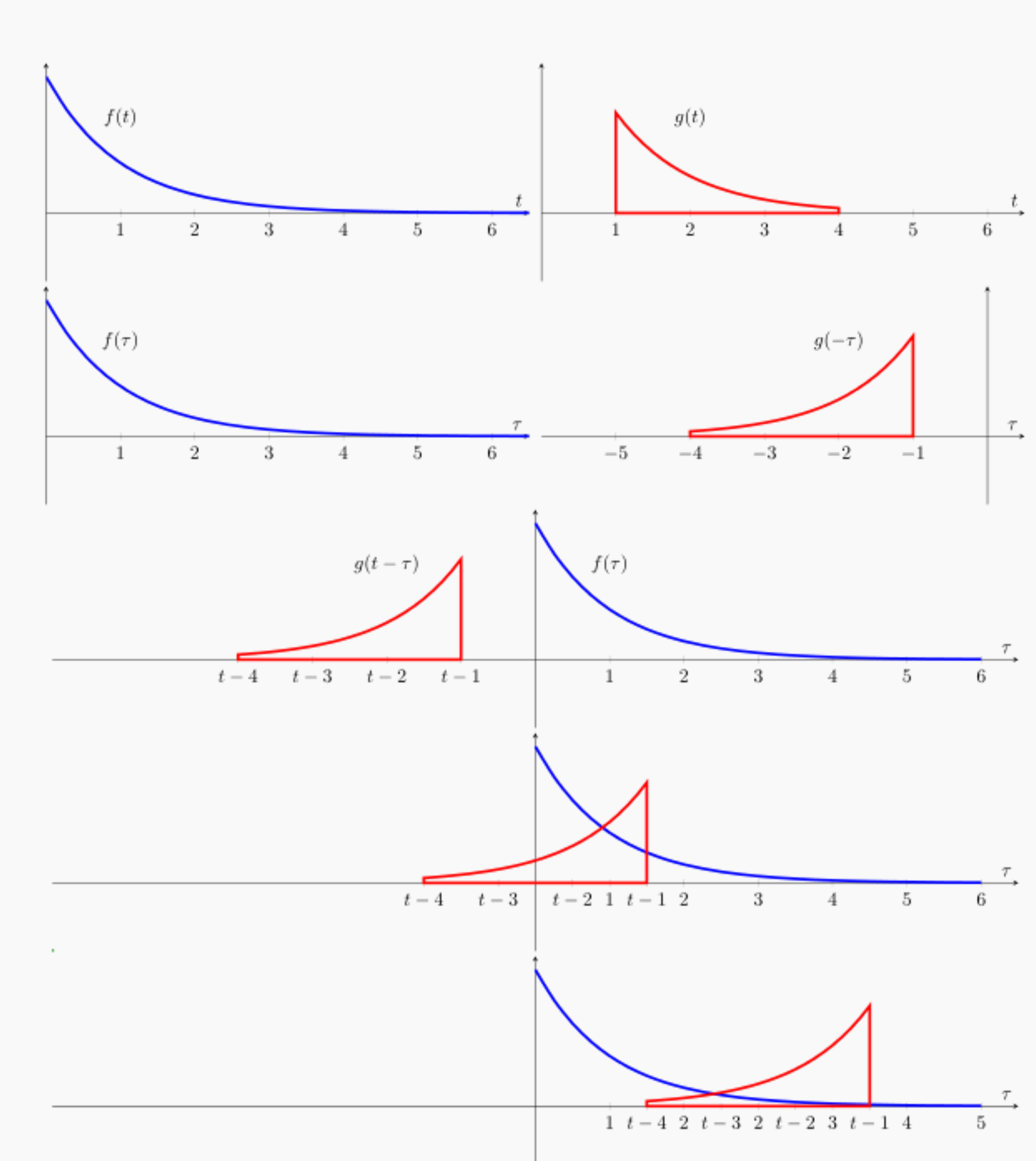
\includegraphics[scale=0.4]{TimeFlipConv.png}
\caption{Convolution slides and sums over a time reversed copy of $h[n]$}
\end{figure}
\end{center}
Since in our case the horizontally flipped version of $h[n]$ will be vertically flipped (negative where it was positive, and vice versa), then multiplying by a flipped and shifted copy is the same as multiplying by a shifted copy - except off by a sign.
\begin{tcolorbox}
So when the following is satisfied:
\begin{align*}
h[a] = -h[L-1 - a]~\forall a \in \mathbb{Z} \\
\end{align*}
then $ACF(h)[n] = -(h*h)[n]$.
\end{tcolorbox}
\clearpage
\section*{Introducing Codes}
\subsection*{Complementary Codes}
We fire two complementary codes $h_1$ and $h_2$ of length $L$ so that $AC(h_1) + AC(h_2) = k\cdot \delta[L-1]$ for some $k \in \mathbb{R}$. The reason we have the spike at $L-1$ is because this is the central element of the autocorrelation of these sequences.
\\\\
We now show this is the case. For a general sequence, when $L = 1$, we have one element in the output autocorrelation. Increasing the length of both of the sequences by one increases the length of the autocorrelation by two, and so the nonzero length of the autocorrelation of a sequence with length $L$ is: $1+2(L-1) = 2L-1$. The first element has index 0 and the last element has index $2L-2$. Therefore, the middle element has index $(0+2L-2)/2 = L -1$.
\section*{Convolving with System Impulse Response}
The output of our system is:
\begin{align*}
y[n] = c_1[n] \star (h[n] * (A \cdot h[n] * c_1[n])) + c_2[n] \star (h[n] * (A \cdot h[n] * c_2[n]))
\end{align*}
where $c_1[n]$ and $c_2[n]$ are a pair of complementary codes, $h[n]$ is the transducer impulse response, and $A \in \mathbb{R}$ captures reflection. Since convolution is commutative, and correlation can be written as a convolution:
\begin{align*}
y[n]/A = (c_1[n] \star c_1[n] + c_2[n] \star c_2[n]) * (h[n] * h[n])
\end{align*}
Call $H[n] = (h*h)[n]$ the impulse response of the ultrasound system, $Y[n] = y[n]/A$ the output normalized per reflection, and $C[n] = c_1[n] \star c_1[n] + c_2[n] \star c_2[n]$ the autocorrelation of the code pair. Then:
\begin{align*}
Y[n] = C[n]*H[n]
\end{align*}
If we define a system $T$ that maps a code autocorrelation to the output, then this system is linear and time invariant, since it is just a convolution with a fixed function:
\begin{align*}
\op{T}{C}[n] \rightarrow C[n] * H[n]
\end{align*}
So, the question for us is: How do we choose a finite symmetric sequence $C[n]$ with a positive peak, so that when we convolve with a symmetric sequence with a negative peak $H[n]$ then we get something very close to a delta function? 
\\\\
One approach would be to add an additional processing step, $P$, so that the final output is:
\begin{align*}
P(\op{T}{C}[n]) = P(C[n]*H[n])
\end{align*} If we choose our codes so that $C[n] = k \cdot \delta[n]$, then we want $P$ to undo the effects of convolving with $H$ - we want it to carry out deconvolution.
\\\\
Also, this implies that if we pick $H[n]$ to be a delta function, then we should decode a delta.
\section*{Repeating Code Elements}
One idea Dr. Zemp had was that by repeating each element in a code, the output should be more peak-like.
\end{document}

















